% BHU PYQ -- Professional Exam Template
\documentclass[11pt,a4paper]{article}

\usepackage[a4paper,top=2.5cm,bottom=2.5cm,left=2.8cm,right=2.8cm,headheight=14pt]{geometry}
\usepackage{amsmath,amssymb}
\usepackage[T1]{fontenc}
\usepackage[utf8]{inputenc}
\usepackage{lmodern}
\usepackage{microtype}
\usepackage{fancyhdr}
\usepackage{enumitem}
\usepackage{hyperref}
\usepackage{lastpage}
\usepackage{parskip}
\usepackage{tikz}
\usetikzlibrary{arrows.meta,shapes,positioning}

\hypersetup{colorlinks=true,urlcolor=black,linkcolor=black,
  pdftitle={B.Sc. (Hons.) Zoology Sem-VI ZOB-602 -- BHU PYQ}}

\pagestyle{fancy}
\fancyhf{}
\renewcommand{\headrulewidth}{0.4pt}
\renewcommand{\footrulewidth}{0.4pt}
\fancyhead[L]{\small\textit{Banaras Hindu University}}
\fancyhead[R]{\small\textit{Zoology Paper: ZOB-602}}
\fancyfoot[C]{\small Page \thepage\ of \pageref{LastPage}}

\newlist{parts}{enumerate}{2}
\setlist[parts,1]{label=(\alph*),leftmargin=*,itemsep=4pt,topsep=3pt}
\setlist[parts,2]{label=(\roman*),leftmargin=*,itemsep=2pt,topsep=2pt}
\newcommand{\pts}[1]{\hfill\textit{[#1]}}

\begin{document}

\begin{center}
  {\large\bfseries BANARAS HINDU UNIVERSITY}\\[2pt]
  {\normalsize B.Sc. (Hons.) Semester VI Examination, 2022-23}\\[6pt]
  \rule{0.8\linewidth}{0.5pt}\\[6pt]
  {\large\bfseries Zoology}\\[4pt]
  {\large\bfseries Paper: ZOB-602 --- Mammalian Endocrinology}\\[4pt]
  {\normalsize Time: Three hours \hfill Full Marks: 70}
\end{center}

\rule{\linewidth}{0.4pt}

\smallskip
\noindent\textit{Note: Answer six questions including Question No. 1 which is compulsory. The figures in the right-hand margin indicate marks.}

\bigskip

\noindent\textbf{Question 1.} Answer the following parts:
\begin{parts}
  \item State whether the following statements are True or False with reason in not more than 2-3 lines each:\pts{$7 \times 2 = 14$}
  \begin{parts}
    \item Higher dopamine level suppresses milk release from lactating female.
    \item SCN, SON, ARC and PVN neurons are located in tuberal region of hypothalamus.
    \item In the pituitary, TRH-R2 mediates the TRH signal.
    \item Relaxin inhibits matrix metalloproteinases and collagenase activity of the pubic symphysis peripartum.
    \item Lutein cells show higher CYP 19 activity as compared to dominant follicular granulosa cells.
    \item Oxytocin exerts myotropic action on the uterus.
    \item Acidosis is one of the factors responsible for hypocalcemic state.
  \end{parts}
  
  \item Define the following:\pts{$6 \times 1 = 6$}
  \begin{parts}
    \item Pentagastrin
    \item KNDy neurons
    \item PNMT
    \item Circadian rhythms
    \item Juxtaglomerular apparatus
    \item Phosphodiesterase.
  \end{parts}
\end{parts}

\medskip\noindent\textbf{Question 2.} The androgen receptor is found in almost every tissue in primates, not just the classical androgen-dependent organs. As a result, androgens have a wide range of effects on a wide range of targets. Discuss.\pts{10}

\medskip\noindent\textbf{Question 3.} Describe in detail the on and off mechanisms of $\text{G}\alpha_{\text{q}}$ signalling pathway.\pts{10}

\begin{center}
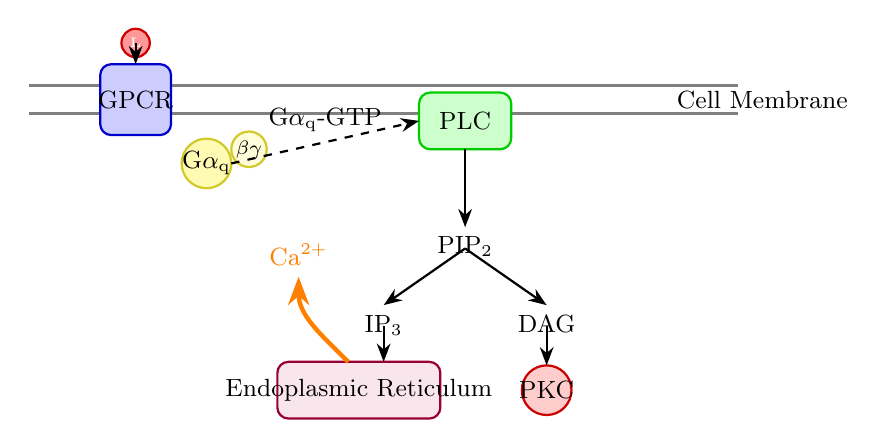
\begin{tikzpicture}[scale=0.9, >=Stealth, every node/.style={font=\small}]
  % Cell membrane
  \draw[very thick, gray] (-5, 2.5) -- (5, 2.5);
  \draw[very thick, gray] (-5, 2.1) -- (5, 2.1);
  \node[right] at (4, 2.3) {Cell Membrane};
  
  % GPCR
  \draw[fill=blue!20, draw=blue!80!black, thick, rounded corners] (-4, 1.8) rectangle (-3, 2.8) node[pos=0.5, align=center] {GPCR};
  \draw[fill=red!40, draw=red!80!black, thick] (-3.5, 3.1) circle (0.2) node[font=\tiny, white] {L};
  \draw[->, thick] (-3.5, 3.1) -- (-3.5, 2.8);
  
  % G-protein
  \draw[fill=yellow!30, draw=yellow!80!black, thick] (-2.5, 1.4) circle (0.35) node {$\text{G}\alpha_{\text{q}}$};
  \draw[fill=yellow!15, draw=yellow!80!black, thick] (-1.9, 1.6) circle (0.25) node[font=\scriptsize] {$\beta\gamma$};
  
  % PLC
  \draw[fill=green!20, draw=green!80!black, thick, rounded corners] (0.5, 1.6) rectangle (1.8, 2.4) node[pos=0.5] {PLC};
  \draw[->, thick, dashed] (-2.15, 1.4) -- (0.5, 2.0) node[midway, above] {$\text{G}\alpha_{\text{q}}\text{-GTP}$};
  
  % PIP2 and split
  \draw[->, thick] (1.15, 1.6) -- (1.15, 0.5);
  \node[below] at (1.15, 0.5) {$\text{PIP}_2$};
  \draw[->, thick] (1.15, 0.2) -- (0.0, -0.6) node[below] {$\text{IP}_3$};
  \draw[->, thick] (1.15, 0.2) -- (2.3, -0.6) node[below] {DAG};
  
  % ER
  \draw[fill=purple!10, draw=purple!80!black, thick, rounded corners] (-1.5, -2.2) rectangle (0.8, -1.4) node[pos=0.5] {Endoplasmic Reticulum};
  \draw[->, thick] (0.0, -0.9) -- (0.0, -1.4);
  \draw[->, ultra thick, orange] (-0.5, -1.4) to[out=135, in=-90] (-1.2, -0.2) node[above] {$\text{Ca}^{2+}$};
  
  % PKC
  \draw[fill=red!20, draw=red!80!black, thick] (2.3, -1.8) circle (0.35) node {PKC};
  \draw[->, thick] (2.3, -0.9) -- (2.3, -1.45);
\end{tikzpicture}
\end{center}

\pagebreak

\medskip\noindent\textbf{Question 4.} Explain the biosynthesis of mineralocorticoids. Comment upon the functions of aldosterone and regulation of its release.\pts{10}

\medskip\noindent\textbf{Question 5.} Write short notes on the following:\pts{$2 \times 5 = 10$}
\begin{parts}
  \item Goitre
  \item Biosynthesis of thyroid hormone
  
  \begin{center}
  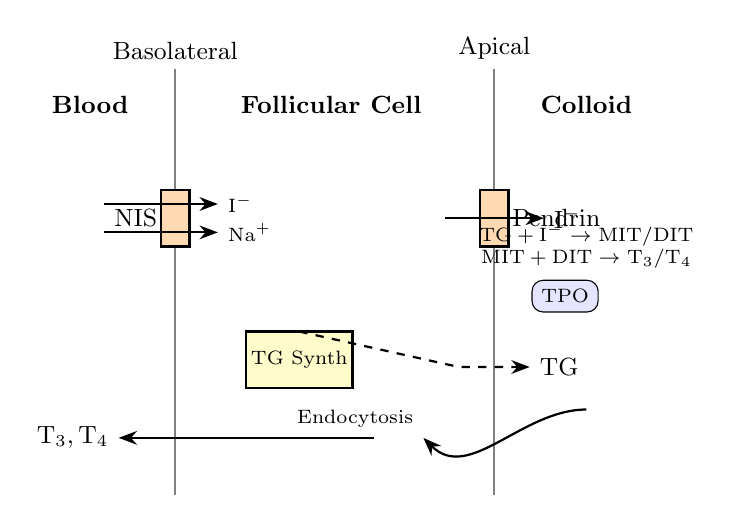
\begin{tikzpicture}[scale=0.9, >=Stealth, every node/.style={font=\small}]
    % Membranes
    \draw[thick, gray] (-3, -3) -- (-3, 3) node[above, black] {Basolateral};
    \draw[thick, gray] (1.5, -3) -- (1.5, 3) node[above, black] {Apical};
    
    % Labels
    \node at (-4.2, 2.5) {\textbf{Blood}};
    \node at (-0.8, 2.5) {\textbf{Follicular Cell}};
    \node at (2.8, 2.5) {\textbf{Colloid}};
    
    % NIS
    \draw[fill=orange!30, thick] (-3.2, 0.5) rectangle (-2.8, 1.3) node[pos=0.5, left=0.1cm] {NIS};
    \draw[->, thick] (-4.0, 1.1) -- (-2.4, 1.1) node[right, font=\scriptsize] {$\text{I}^-$};
    \draw[->, thick] (-4.0, 0.7) -- (-2.4, 0.7) node[right, font=\scriptsize] {$\text{Na}^+$};
    
    % Pendrin
    \draw[fill=orange!30, thick] (1.3, 0.5) rectangle (1.7, 1.3) node[pos=0.5, right=0.1cm] {Pendrin};
    \draw[->, thick] (0.8, 0.9) -- (2.2, 0.9) node[right] {$\text{I}^-$};
    
    % TG
    \draw[fill=yellow!20, thick] (-2, -1.5) rectangle (-0.5, -0.7) node[pos=0.5, font=\scriptsize] {TG Synth};
    \draw[->, thick, dashed] (-1.25, -0.7) -- (1.0, -1.2) -- (2.0, -1.2) node[right] {TG};
    
    % TPO
    \node[draw, fill=blue!10, rounded corners, font=\scriptsize] at (2.5, -0.2) {TPO};
    \node[font=\scriptsize, align=center] at (2.8, 0.5) {$\text{TG} + \text{I}^- \rightarrow \text{MIT/DIT}$ \\ $\text{MIT} + \text{DIT} \rightarrow \text{T}_3/\text{T}_4$};
    
    % Endocytosis
    \draw[->, thick] (2.8, -1.8) to[out=180, in=-45] (0.5, -2.2) node[above left, font=\scriptsize] {Endocytosis};
    \draw[->, thick] (-0.2, -2.2) -- (-3.8, -2.2) node[left] {$\text{T}_3, \text{T}_4$};
  \end{tikzpicture}
  \end{center}
\end{parts}

\medskip\noindent\textbf{Question 6.} Discuss how the hypothalamus serves as the major regulator of the adenohypophysis.\pts{10}

\pagebreak

\medskip\noindent\textbf{Question 7.} Describe the biosynthesis and biological actions of melatonin.\pts{10}

\begin{center}
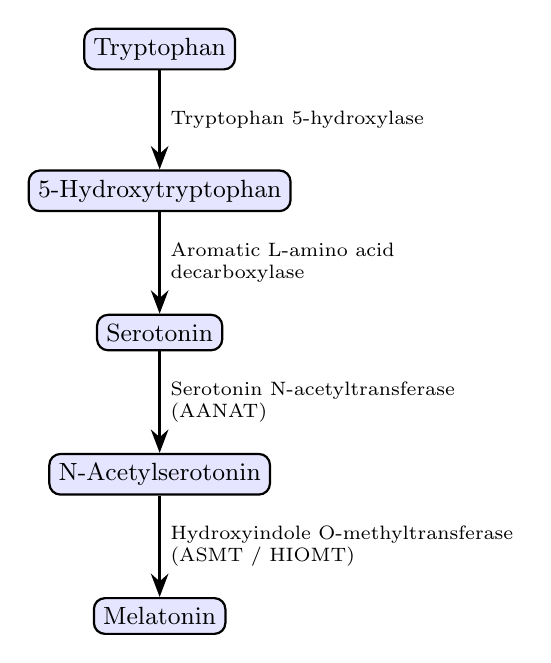
\begin{tikzpicture}[scale=0.9, >=Stealth, every node/.style={font=\small}]
  \node[draw, fill=blue!10, thick, rounded corners] (tryp) at (0, 4) {Tryptophan};
  \node[draw, fill=blue!10, thick, rounded corners] (htp) at (0, 2) {5-Hydroxytryptophan};
  \node[draw, fill=blue!10, thick, rounded corners] (sero) at (0, 0) {Serotonin};
  \node[draw, fill=blue!10, thick, rounded corners] (nas) at (0, -2) {N-Acetylserotonin};
  \node[draw, fill=blue!10, thick, rounded corners] (mela) at (0, -4) {Melatonin};
  
  \draw[->, very thick] (tryp) -- (htp) node[midway, right, align=left, font=\scriptsize] {Tryptophan 5-hydroxylase};
  \draw[->, very thick] (htp) -- (sero) node[midway, right, align=left, font=\scriptsize] {Aromatic L-amino acid\\decarboxylase};
  \draw[->, very thick] (sero) -- (nas) node[midway, right, align=left, font=\scriptsize] {Serotonin N-acetyltransferase\\(AANAT)};
  \draw[->, very thick] (nas) -- (mela) node[midway, right, align=left, font=\scriptsize] {Hydroxyindole O-methyltransferase\\(ASMT / HIOMT)};
\end{tikzpicture}
\end{center}

\medskip\noindent\textbf{Question 8.} A person is diagnosed with hyperglycemia, glycosuria and polydipsia. Give an account of the hormonal dysfunction and mechanism of pathophysiological consequences.\pts{10}

\vfill
\rule{\linewidth}{0.4pt}
\begin{center}\small
\href{https://bhu-exam.vercel.app/}{Click Here}\\[4pt]\href{https://me-aryan.vercel.app/}{Click Here}\\[4pt]\href{https://quashan-me.vercel.app/}{Click Here}
\end{center}

\end{document}
